\section{電流パルスを用いたパルス加熱・急冷実験の手法}
%相転移の実験は光学クライオスタット中のヘリウムガス
本章では電流パルスを用いた半導体スズから金属スズへの変換と共存状態生成に関する実験手法について説明する。

\subsection{Sn-Ge合金への端子付け}
まずパルス印加実験に先立って、Sn-Ge試料に4つの電極端子を付けた。
本節では端子付けに用いた道具と標準的な端子付けの手順、注意事項を述べたあと、パルス印加実験に用いる端子付け手法を述べる。

\subsubsection{端子づけに用いた道具}
端子付けには以下を用いた。
\begin{itemize}
\item 乾いた毛筆($250\mu m$程度)
\item 乾いた毛筆($500\mu m$程度)
\item 毛筆(銀ペースト用)
\item 毛筆(カーボンペースト用)
\item 毛筆(グリース用)
\item 銀ペーストを練るようじ
\item カーボンペーストを練るようじ
\item ピンセット
\item キムワイプ
\item 金線(太さ25um)
\item 金線(太さ50um)
\item 銀ペースト
\item カーボンペースト
\item コハク酸ジエチル
\item ワニス
\item 光学顕微鏡
\item 金線を切るためのハサミ
\item 金線を置いておくゴムマット
\item 銀ペーストを練るスライドガラス
\item カーボンペーストを練るスライドガラス
\item ユニバーサル基盤(ピッチ2.5mm)
\item サファイア基板
\item 両面テープ
\end{itemize}

毛筆とはつまようじの先に一本の毛を取り付けたもので、太さと長さが異なったものを用途により使い分けた。毛の長さを長くしすぎると試料や金線を飛ばしてしまうことに注意する。

毛筆を作るときは、二液式接着剤を混ぜてつまようじの先に薄くつけ、一本の毛(腕毛、すね毛、まつげ、髪の毛など)を、接着剤に先を出して埋め込む。接着剤が乾いたら、毛の長さをはさみで調整した。
 
\subsubsection{四端子付けの手順} 
まず準備段階ではユニバーサル基盤やサファイア基板を適当な大きさにカットし、簡単に動かないようにスライドガラスに両面テープで固定した。このとき銀ペーストを伸ばすパレットを横に作ると便利である。さらに金線を必要なぶん切っておき(まっすぐで長さのそろった、汚れていないものが扱いやすい)、ゴムマットの上で軽く曲げた。冷却・加熱時には収縮・膨張によってサンプルと端子には応力がかかり、それが端子が外れる原因となった。金線の曲げは応力を緩和するために一定の効果がある。銀ペーストをよく練って、サンプル横のパレットに適量のせた。銀ペーストの粘度は作業効率と端子の強度に直結するため特に注意する。
 
つぎにサンプルを仮留めした。まず基板にグリースを毛筆でごく少量つける。このグリースを毛筆で伸ばす必要はない。そして毛筆の先にグリースを微量つけてサンプルを持ち上げ、ユニバーサル基板につけたグリースの上に置いた。このサンプルを上から乾いた毛筆で軽く押して、密着させた。
 
仮止めの後は2本の電流端子をサンプルにつけた。まず(曲がった)金線一本をピンセットと乾いた毛筆で移動し、一方の端がサンプルの近くでもう一方がプローブ側の端子(銅線の足やユニバーサル基板の銅箔)の近くにくるようにした。このときは金線にはまだ銀ペーストをつけていない。次に金線とプローブ側の端子を銀ペーストでくっつけた。同時に金線のもう一方がサンプルに触れるように微調整し、固まるまで待った。もう一本の金線に関しても同様に、プローブ側の端子と金線を銀ペーストでくっつけて固まるまで待った。銀ペーストが固まったらサンプルと金線を銀ペーストでつないだ。流れる電流がなるべく一様な密度になるように、横に広く接続することを意識した。パルス印加実験の際も同様に電流端子を接続したが、後述するようにカーボンペーストを一部に用いた点が異なる。
 
サンプルと金線の間の銀ペーストが固まったら、金線と基板の間に毛筆を入れてサンプルを持ち上げ、浮いた状態とする。これはサンプルに応力がかからないようにするためと、熱的な接触を避けるためである。
 
次に電流端子で支えられ浮いた状態のサンプルについて電圧端子を接続した。端子付け法は電流端子と同様である。ただし銀ペーストがサンプルに触れる面積が小さくなるように心がけた。電流端子に用いる金線も電流端子のものと同様に折り曲げて使うと

最後に記録のため写真をとり、導通を確認した。端子間の抵抗は物質により異なるが、スズやIrTe$_2$の場合数$\Omega$程度が典型的だった。
 
\subsubsection{作業のコツ・注意事項} 
本節では作業の際の技術的なコツと注意した点に関して筆者の考えを述べる。

ピンセットは細かな作業の際に重要な役割を果たす。汚れたらキムワイプで拭いて先を綺麗に保つことが大切である。精密なピンセット先を保護するために、金線はゴムマットの上でつまむ。
 
毛筆を使うときも、ピンセットと同様に先を綺麗に保つことが重要である。銀ペーストを塗ったあとは毎回毛を溶媒のコハク酸ジエチルで洗って、キムワイプで拭くとよいことがわかった。毛筆を持つときはつまようじを人差し指と中指で持つと疲れにくい。また小指の付け根を台につけて左手を添えると震えにくい。

金線はつよく掴むと形が変わってしまうため、できるだけピンセットで平行につまむことを心がけた。

銀ペーストの粘度を十分に高くすると、乾くのにかかる時間を短くできるため作業効率と直結する。また端子の機械的な強度を上げることにもつながる。
溶媒(コハク酸ジエチル)の液溜まりと固い銀ペーストの塊はスライドガラス上に離しておき、適宜混ぜながら使うと粘度を調整しやすい。小さなサンプルと金線を接続するときはまず薄い銀ペーストの表面張力でくっつけるとよい。乾くのを待って、濃いペーストで形を整える。はみ出した時は細く切った(2$\sim$20mm)キムワイプの先をちぎってねじったものに溶媒(コハク酸ジエチル)を含ませて拭く。

顕微鏡の倍率は高倍率で固定して毛筆やピンセットはなるべく動かさず、スライドガラスとサンプルを動かすようにするとよい。

測定中に端子が外れたときは原因の究明のために測定後の光学顕微鏡像の画像をとって、測定前と比べてみるとよい。各端子間の抵抗を測ってみたり毛筆で端子を触ってみると、どの端子が外れたか分かる。

端子付けには集中を要するので、一時間半に少なくとも一度休憩するのが望ましい。
前日はよく寝て、机の上を整理整頓することも注意が散漫にならないようにするために重要である。また直前の激しい運動は控えるとよいらしい。
空調の風で金線が飛ぶことがあるのでここぞというときは空調のスイッチを切るとよい(作業終了後は再度スイッチを入れる)。 椅子の高さ、左右の接眼レンズの間隔とピントを調整するくせをつけることも有益である。

\subsubsection{電流パルス実験の際の技術的な工夫} 
スズの相転移には大きな体積変化が伴うため、電流パルスにより試料の温度を上げて相転移を起こし、端子がくっついた状態を維持するためにはいくつかの技術的な工夫が欠かせない。本節ではその技術的な工夫とその手法に至るまでの失敗例を説明する。

まず本実験に用いた成功例を述べる。筆者は図\ref{fig:schematics_sample}のような端子の接続法を見出した。カーボンペーストは発熱に十分に高い抵抗が実現できる一方で機械的な強度が低く、銀ペーストは強度が高い一方で抵抗が小さい。これらを効果的に組み合わせることで、筆者は機械的強度と高抵抗を確保できると筆者は考えた。そこでカーボンペーストで金線をコーティングした後、銀ペーストで覆い試料にしっかりと接続した。この構成では低抵抗率の銀ペーストが挟まっているので試料と金線の間に電流経路が集中せず、比較的一様な発熱が可能となったと考える。また電流端子につなぐ金線は1A程度以下の電流で焼き切れないように直径$\rm 50 \mu m$のものとした。一方電圧端子をつなぐ線には大電流が流れないため、試料に応力をかけないよう柔らかく、熱伝導の高すぎないものとしたかった。そこで直径$\rm 25 \mu m$の金線とした。
\begin{figure}[!h]
    \begin{center}
   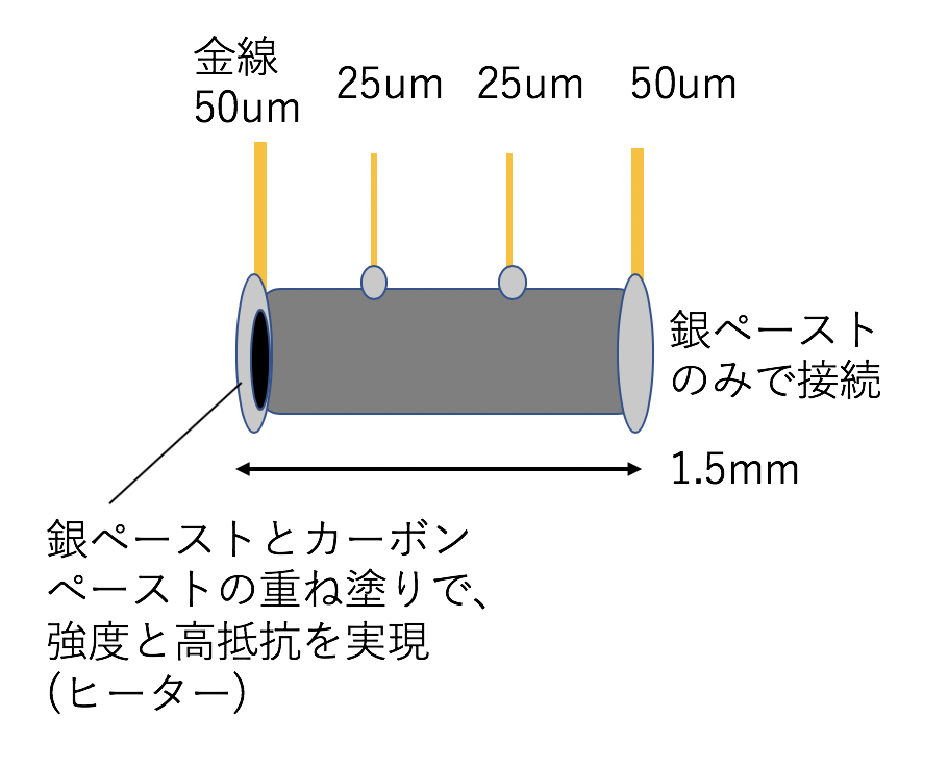
\includegraphics[width=0.4\hsize]{experiment/schematics_sample.eps}
  \end{center}
  \caption{実験に用いた接続法}
  \label{fig:schematics_sample}
\end{figure}

次に失敗例を述べる。まずファーストトライアルにおいて、筆者は直径$\rm 25 \mu m$の金線を電圧・電流端子として銀ペーストで試料に接続した。その試料を25Kに保持し電流パルスを印加したところ、試料が相転移温度に達するまえに直径$\rm 25 \mu m$の金線からなる電流端子が焼き切れた。そのときの電流は1.3A程度だった。したがって電流端子に繋ぐ金線は$\rm 25 \mu m$より太いものに取り替える必要がある。また数A程度の電流を流すと試料付近以外でも発熱し断線のリスクがあるため、あえて試料付近に高抵抗(ヒーター)の領域を作って発熱効率を高める必要がある。

そこで、次に筆者はカーボンペーストで直径$\rm 50 \mu m$の金線を接続することで、高抵抗のカーボンペーストで効果的に試料を加熱しながら、かつ金線が焼き切れないような構成を目指した。しかしこの構成では試料が相転移温度に達するまえに、カーボンペーストによる接続部が過熱で壊れてしまった。この結果はカーボンペーストは銀ペーストに比べ抵抗が高い反面、機械強度が弱いことに起因する。またカーボンペーストを用いた電気的な接続では、カーボンペーストの高い抵抗率に起因して発熱部分が試料と金線の間に集中してしまう。

\subsection{半導体スズから金属スズへの変換}
まずパルス印加の前に抵抗の温度依存性も測定した。抵抗の温度依存性を測定するときの電気回路の模式図を図\ref{fig:schematics_lockin}に示す。ロックインアンプ(Stanford Research SR830)から出力した105Hzの正弦波の交流電圧は、光学クライオスタット中の試料とロード抵抗の直列接続に印加される。回路に流れる電流は$\rm 150\Omega$のロード抵抗の電圧降下をマルチメータ(Keithley 2001)で読み取り算出した。試料の電圧端子間の電圧効果はトランス増幅器(Stanford Research SR554)で100倍に増幅したあと、ロックインアンプの入力端子に入力した。回路に流す電流値は、25Kの試料で温度上昇が認められなかった値より十分小さくとった。また試料の複素インピーダンスの虚部(位相進み/遅れ)成分は実部の1/100程度以下だったので無視して、実部のみを抵抗とした。
\begin{figure}[!h]
     \begin{center}
   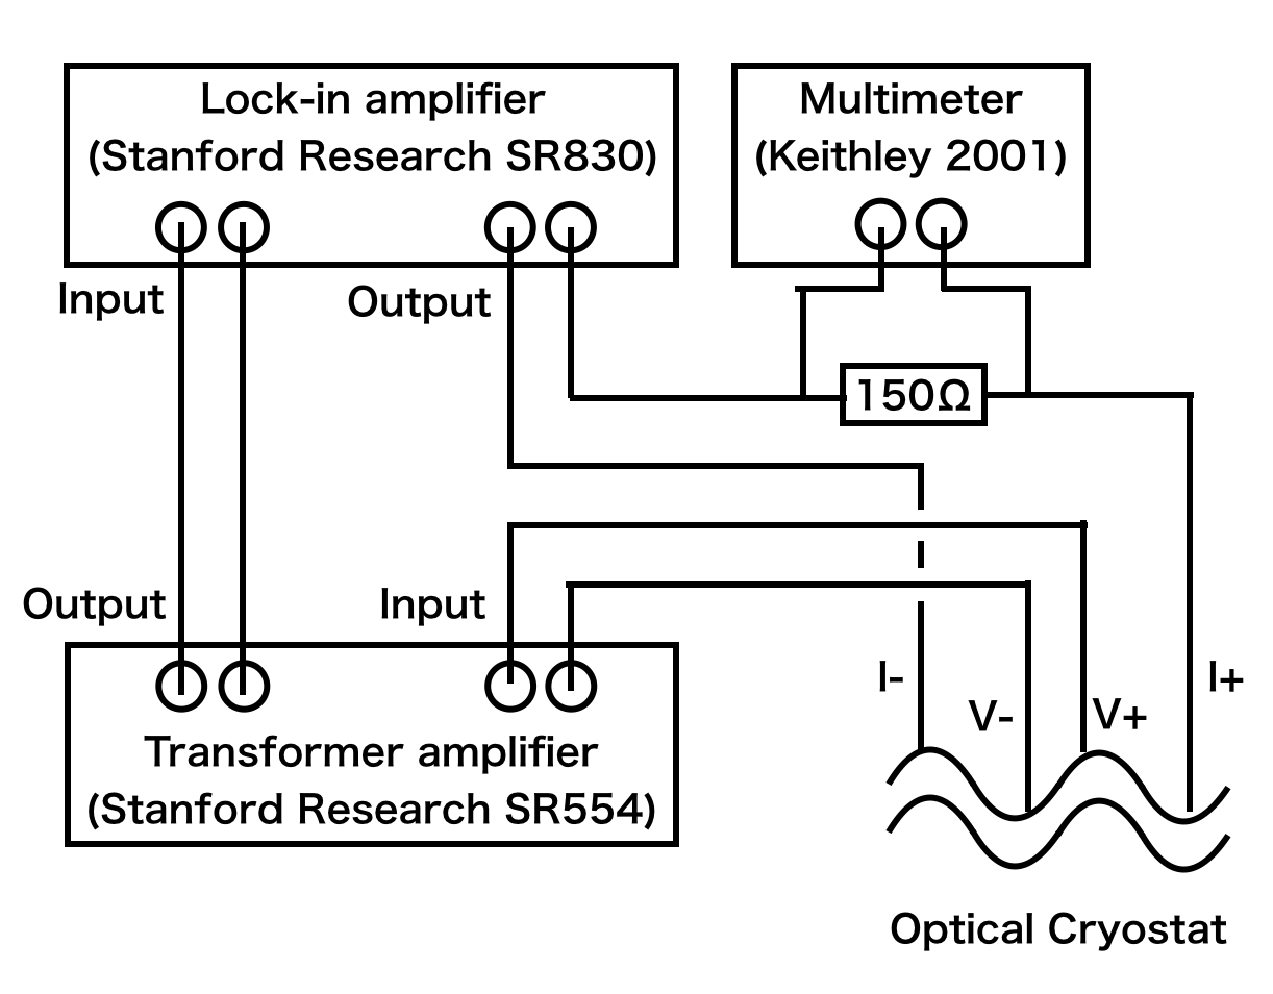
\includegraphics[width=0.5\hsize]{experiment/schematics_lockin.eps}
  \end{center}
  \caption{}
  \label{fig:schematics_lockin}
\end{figure}

試料への端子接続は前節で述べた手法を用いた。

抵抗の温度依存性を測定した後αスズからβスズに相転移を起こすことを目的として、25Kに保った試料に孤立した矩形波の電流パルスを3秒印加してジュール発熱により加熱した。スズ相転移前後で抵抗が大きく異なるため、相転移の確認はパルス印加中の抵抗変化を測定することで行った。その際用いた電気回路の模式図を図\ref{fig:schematics_pulse}に示す。ソースメータ(Keithley 2400)から出力されたパルス電圧は、パワーアンプ(NF Corp. 4502)で100倍に増幅されたあと、光学クライオスタット中の試料とロード抵抗の直列接続に印加される。回路に流れる電流の時間変化は、$\rm 5.4\Omega$のロード抵抗の電圧降下をデータロガー(MC DT8824)で読み取り計算した(Ch2)。また試料の電圧降下もデータロガー(MC DT8824)で読み取り計算した(Ch1)
\begin{figure}[!h]
    \begin{center}
   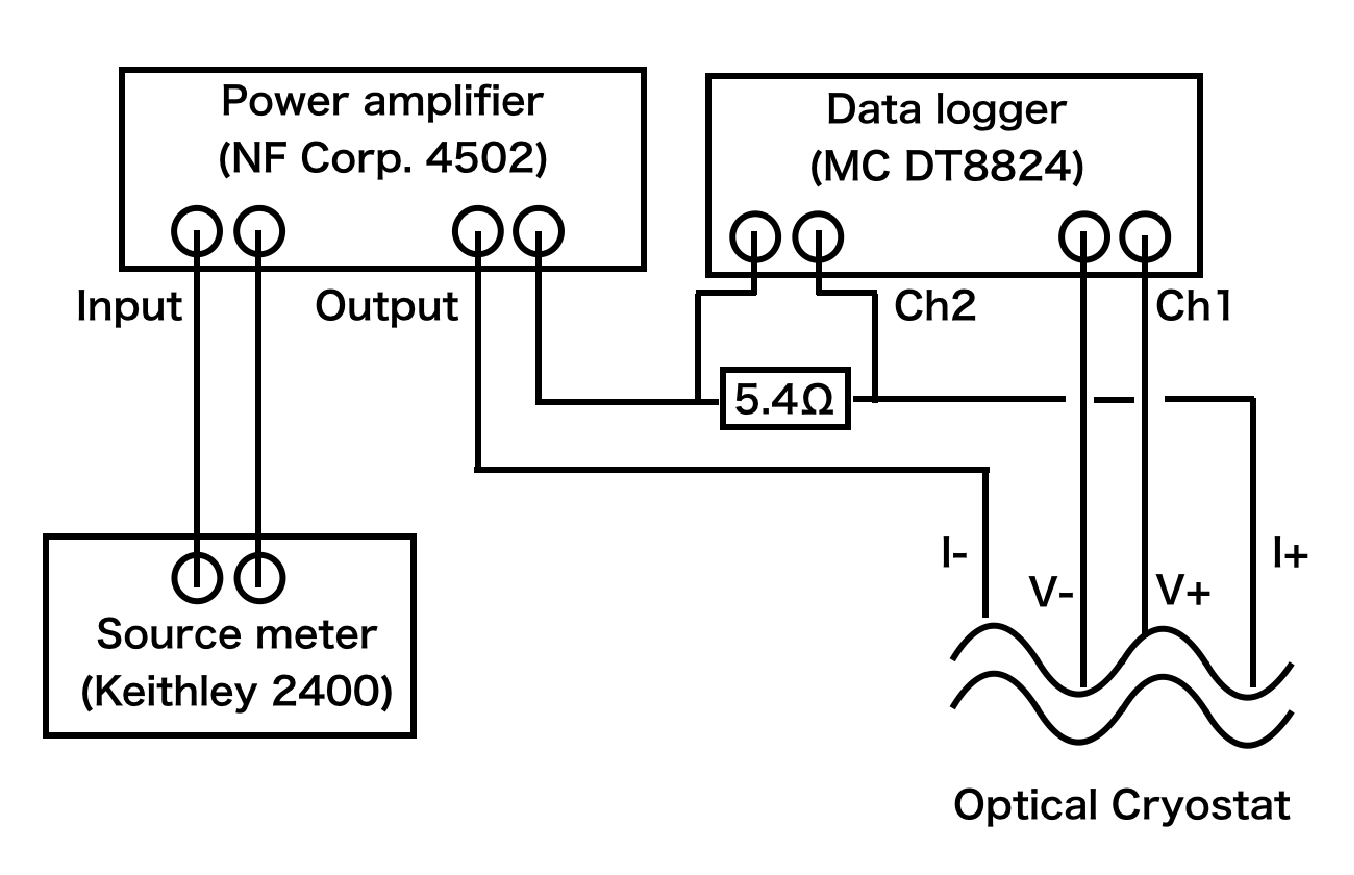
\includegraphics[width=0.5\hsize]{experiment/schematics_pulse.eps}
  \end{center}
  \caption{}
  \label{fig:schematics_pulse}
  \end{figure}
  
%効果的に試料を加熱するために筆者は図\ref{fig:schematics_sample}のような端子の接続法を用いた。\ref{sec:4terminal}に述べるように、カーボンペーストは発熱に十分に高い抵抗が実現できる一方で機械的な強度が低く、銀ペーストは強度が高い一方で抵抗が小さい。これらを効果的に組み合わせることで、筆者は機械的強度と高抵抗を確保できると筆者は考えた。そこでカーボンペーストで金線をコーティングした後、銀ペーストで覆い試料にしっかりと接続した。この構成では低抵抗率の銀ペーストが挟まっているので試料と金線の間に電流経路が集中せず、比較的一様な発熱が可能となったと考える。また電流端子につなぐ金線は1A程度以下の電流で焼き切れないように直径$\rm 50 \mu m$のものとした。一方、電圧端子をつなぐ線には大電流が流れないため、柔らかく熱伝導の高すぎないものとしたかった。そこで直径$\rm 25 \mu m$の金線とした。

電流パルスを印加した後にふたたび試料抵抗の温度依存性を測定した。パルス印加前と同様に図\ref{fig:schematics_lockin}の電気回路を用いた。

\subsection{半導体スズと金属スズの共存状態の制御}
次に電流パルスを印加してαスズを部分的にβスズに変換し、αスズとβスズの共存状態を生成することを目指した。序論で述べた通りαスズとβスズはともに温度200K以下と室温で安定である。室温でもパルス印加で相転移が示せれば極めて有用と筆者は考える。さらに低温での実験に比べ冷媒を必要とせず、簡便で実験の自由度も大きい。そこで本実験では室温に保った試料に電流パルスを印加した。

本実験に用いた電気回路は前節のパルス印加実験と同様である。ただし図\ref{fig:schematics_sample2}のように電流端子の片側のみにカーボンペーストを用いた点が異なる。主に片側のみから発熱させることで意図的に試料内の温度勾配を作り出し、部分的な書き込みを制御した。カーボンペーストを用いて接続する方法は前節と同様である。
\begin{figure}[!h]
 \begin{minipage}{0.5\hsize}
    \begin{center}
   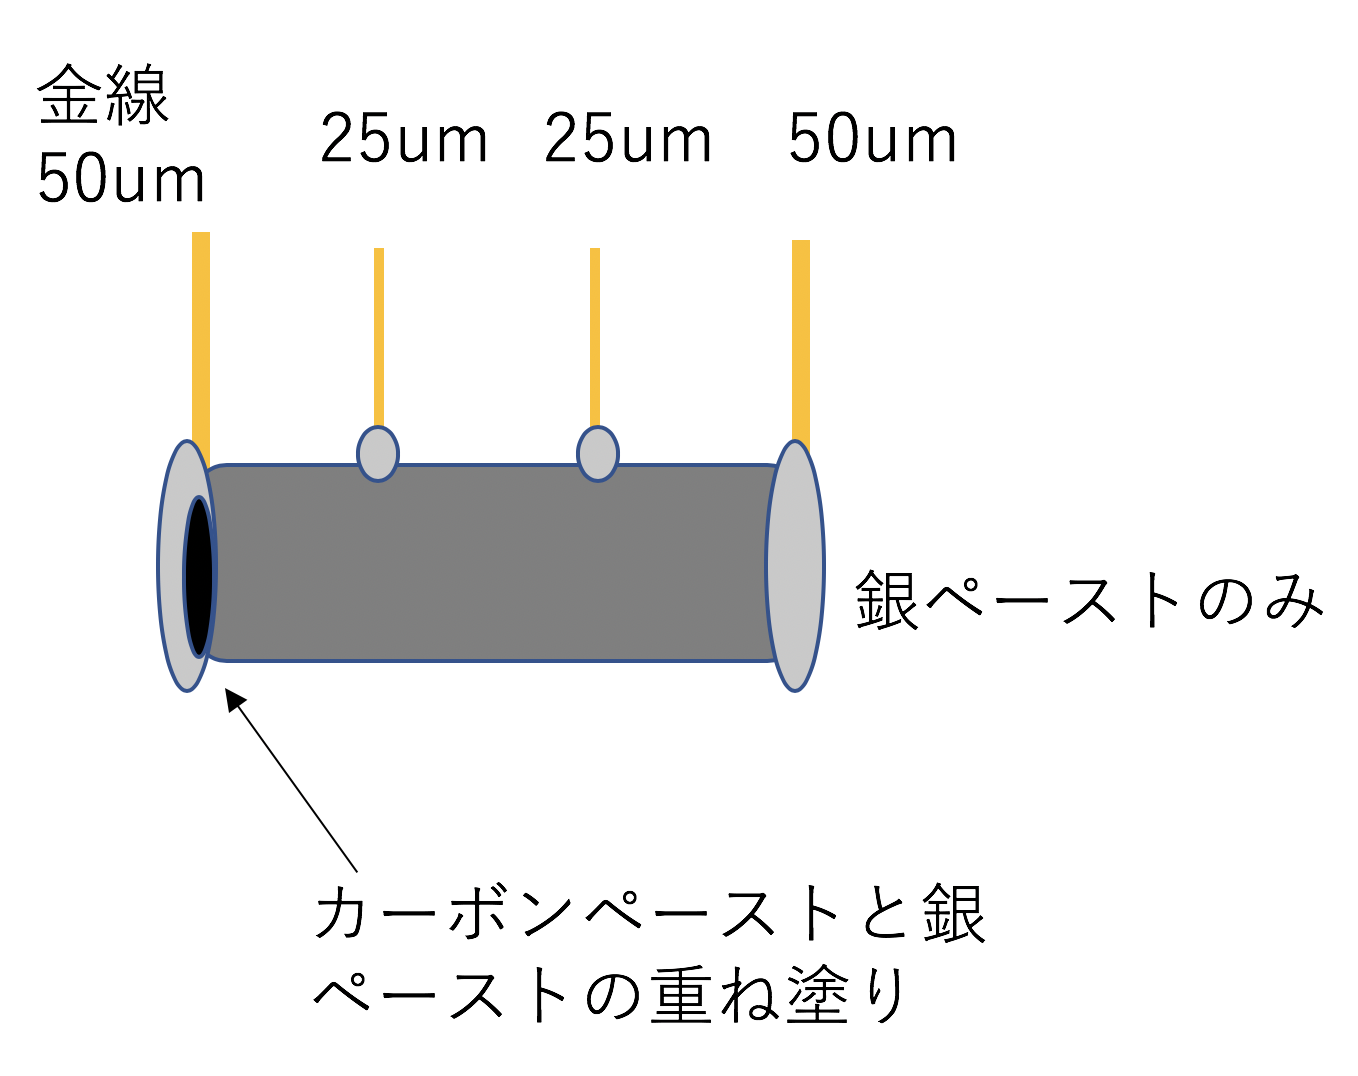
\includegraphics[width=0.9\hsize]{experiment/schematics_sample2.eps}
  \end{center}
  \caption{}
  \label{fig:schematics_sample2}
   \end{minipage}
 \begin{minipage}{0.5\hsize}
    \begin{center}
   \includegraphics[width=0.8\hsize]{experiment/microscope.eps}
  \end{center}
  \caption{}
  \label{fig:microscope}
   \end{minipage}
\end{figure}

また顕微光学系を構成し、パルス印加中の試料を光学的に観察した。図\ref{fig:microscope}に顕微光学系の模式図を示す。光源から照明を入射する際に、顕微光学系の光軸から外した配置とすることで迷光を抑え、コントラストの大きな動画・画像を撮影した。


本実験ではパルス幅1秒、インターバル1秒のパルス列を試料に印加した。

%\subsection{電流パルスを用いたβ相からα相への変換}

\clearpage

%\ref{sec:4terminal}